\documentclass[12pt, a4paper]{article}
\usepackage{graphicx}
\graphicspath{{images/}}

\title{My First LaTeX document}
\author{Asif Shahriar\thanks{Funded by Overleaf team.}}
\date{May, 2023}


\begin{document}
\maketitle
First document. This is a simple example, with no extra parameters
or packages included.We have now added a tiltle, author and date 
to our first \LaTeX{} document!

%This line here is a comment. It will not be typeset in the document. 

Some of the \textbf{greatest} discoveries in \underline{science}
were made my \textbf{\textit{accident}}. 

Some of the greatest \emph{discoveries} in science were made by
accident. 

\textit{Some of the greatest \emph{discoveries} in science were
made be accident.}

\textbf{Some of the greatest \emph{discoveries} in scince were made
by accident.}

The universe is immense and it seems to be homogeneous, on a large
scale, everywhere we look. 

%The \includegraphics command is provided (implemented) by the 
% graphics package

\begin{figure}[h]
    \centering
    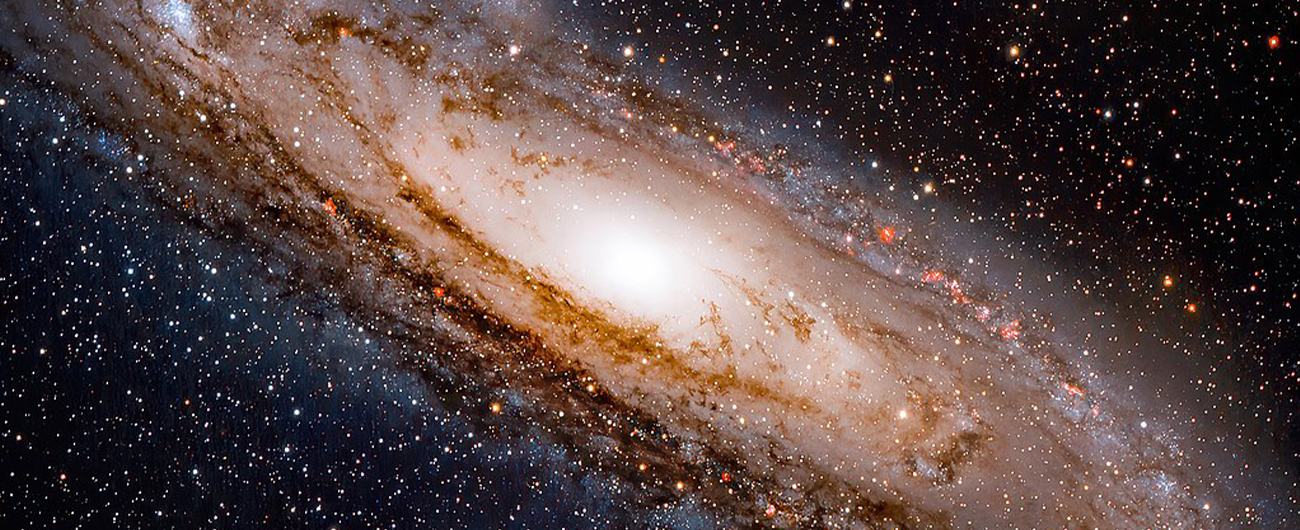
\includegraphics[width=0.75\textwidth]{universe}
    \caption{A picture of universe}
    \label{fig:universe1}
\end{figure}

As you can see in figure\ref{fig:universe1}, the function grows near
the origin. This example is on page\pageref{fig:universe1}. 


\end{document}
